\documentclass[a4paper,11pt, twocolumn]{article}
%\usepackage[T1]{fontenc} %for å bruke æøå
\usepackage[utf8]{inputenc}
\usepackage[T1]{fontenc}
\usepackage[norsk]{babel}
\usepackage{graphicx} %for å inkludere grafikk
\usepackage{verbatim} %for å inkludere filer med tegn LaTeX ikke liker
\usepackage{mathpazo}
\usepackage{mathtools}
\usepackage{csquotes}
\usepackage{tikz}
\usepackage{listings}
\usepackage{booktabs}
\usepackage{todonotes}
\usepackage[backend=biber]{biblatex}
\usepackage{caption} 
\usepackage{parboxx}
\hyphenpenalty=750
\captionsetup[table]{skip=10pt}

\addbibresource{elastisitet.bib}


\lstset{language=Matlab, commentstyle=\textcolor[rgb]{0.00,0.50,0.00}, keepspaces=true, columns=flexible, basicstyle=\footnotesize, keywordstyle=\color{blue}, showstringspaces=false, inputencoding=ansinew}

\title{Rapport 4 FYS2150\\Elastisitet}

\author{Eivind Brox}
\date{\today}

\begin{document}
\maketitle


\begin{abstract}
I denne rapporten undersøker vi to metoder for å finne elastisitetsmodulen til materialet i en messingstav. Elastisiteten er en nyttig egenskap som gir oss ny informasjon i forhold til bruksområdet til materialet. 

Vi finner en elastisitetsmodulus på $104.6\pm0.3$GPa ved å måle defleksjonen til en messingstav, og $103.5\pm0.1$GPa ved å måle svingefrekvensen til samme stav ved opptak av lyd og fouriertransformasjon.

Vi finner at det dobbelte av usikkerheten i differansen er mindre enn differansen selve differansen. Vi konkluderer med at det virker som om den faktoren som gjør seg mest gjeldene for dette er at vi trodde oppsettet var riktig når vi kom på laben, og glemte å undersøke om defleksjonsmålingene ble gjort akkurat på midten av punktene staven hvilte på.

\end{abstract}

\section{Introduksjon}
Elastisiteten til materialer er en egenskap som er interessant i mange sammenhenger. Den elastisiteten vi undersøker i denne rapporten handler om egenskapen som forteller i hvilken grad materialet vårt oppfører seg når det påtrykkes en kraft, og hvordan det går tilbake til utgangspunktet når kraften fjernes. Vi ser bare på områder der materialet oppfører seg normalt, og ikke de ekstreme tilfelle der materialet deformeres så kraftig at det ikke beveger seg tilbake til utgangsposisjonen.

Når vi har elastisitetsmodulen til et materiale, i tillegg til andre grunnleggende egenskaper, har vi informasjon som kan forteller oss noe nytt om bruksområdet. Elastisiteten er en essensiell egenskap som spiller en viktig rolle for mange applikasjoner. Alt fra bygging av skyskrapere til konstruksjon av kulepenner, og det som mindre er.

I denne rapporten introduseres først teorien for de to forskjellige metodene som er benyttet for å estimere elastisitetsmodulen. Vi har benyttet defleksjon av stav og måling av materialets svingefrekvens for å estimere modulen. Videre presenteres hvilket utstyr som er benyttet, hvordan dette er satt opp og hva som er gjort for å utføre målingene. Resultatene presenteres før de er vurdert og en konklusjon trekkes til slutt. 
  
\section{Teori}
Vi ønsket å måle elastisitetsmodulen både ved å se på hvor mye en sylinderstav bøyde seg ved påtrykt kraft, og ved å undersøke hvilken grunnfrekvens staven stabiliserte seg på en stunde etter vi hadde påført en impuls for å sette den i vibrasjon.
\subsection{Nedbøying av stav}
Fra oppgaveteksten for det eksperimentelle arbeidet, \cite{oppgavetekst}, har vi at defleksjonen, $h(m)$, for en bjelke støttet på to punkter, med belastning midt mellom disse punktene er

\begin{equation}
	h(m) = \frac{mgl^3}{48EI}
	\label{eq:h}
\end{equation}

Der $mg$ er kraften som virker midt bjelken, $l$ er avstanden mellom punktene bjelken hviler på, $E$ er elastisitetsmodulen og $I$ er andre arealmoment. For en sylinder har vi

\begin{equation}
	I = \frac{\pi d^4}{64}
\end{equation}

Defleksjonen oppfører seg tilnærmet lineært, og finner vi stigningstallet for lineærtilpasningen av målingene våre, $A$, kan vi uttrykke elastisitetsmodulen som  

\begin{equation}
	E = \frac{4l^3g}{3\pi |A|d^4}
	\label{eq:elastisitetsmodulDefleksjon}
\end{equation}

Vi får en usikkerhet på
\begin{equation}
	s_E = E\sqrt{\left(\frac{s_A}{A}\right)^2+\left(\frac{4s_d}{d}\right)^2+\left(\frac{3s_l}{l}\right)^2}	
	\label{eq:feilDefleksjon}
\end{equation}


\subsection{Dynamisk bestemmelse av elastisitetsmodulen ved måling av lydhastighet}
Teorien er også her hentet fra oppgaveteksten \cite{oppgavetekst}. 

Ved å utnytte at elastisitetsmodulen for et material avhenger av hastigheten til lyden i materialet og tettheten til materialet på følgende måte

\begin{equation}
	E = \rho v^2
	\label{eq:dynamiskElastisitet}
\end{equation}

kan vi ved relativt enkle målinger finne et estimat for elastisitetsmodulen. Her er $v$ utbredelseshastigheten for de longitudinale bølgene i materialet vårt og $\rho$ er tettheten til materialet.

Vi utnytter at bølgelengden, $\lambda$, for de longitudinale bølgene for en stav kan beskrives ved 

\begin{equation}
	\lambda = \frac{2L}{n}, \quad n = 1, 3, 5, \dots
\end{equation}

der $L$ er stavens lengde. Vi vet at frekvensen, $f$, er beskrevet ved $f = v/\lambda$, slik at vi får 

\begin{equation}
	v = 2Lf
\end{equation}

ettersom svingningene ved de lengste bølgelengdene er de som dempes saktest. Vi kan dermed uttrykke elastisitetsmodulen som

\begin{equation}
	E = 4\rho(Lf)^2
	\label{eq:dynEl}
\end{equation}

Vi får en usikkerhet på
\begin{equation}
	s_E = E\sqrt{\left(\frac{2s_d}{d}\right)^2+\left(\frac{2s_f}{f}\right)^2+\left(\frac{s_L}{L}\right)^2+\left(\frac{s_m}{M}\right)^2}	
	\label{eq:feilDynamisk}
\end{equation}

Vi kan bytte ut tettheten i ligning \eqref{eq:dynEl} med formelen for tettheten til en sylinder, og få

\begin{align}
	E &= \frac{16Lf^2M}{\pi d^2}
\end{align}

der $M$ er massen til sylinderen. Dette gjelder for  

\section{Eksperimentelt}
{\bf Utstyr:}

Dimensjoner messingstav og defleksjonsmålinger:
\begin{itemize}
	\item Målebånd, Laufkin 2m Pee Wee Y612CM
	\item Mikrometer, Moore and Wright
	\item Messingstav
	\item Kalibreringslodd: 2kg, 1kg, 100g og 10g
	\item Balansevekt, Ohaus
	\item Stativ med kniver og oppsett for måleur
	\item Skrutrekker
\end{itemize}

Dynamisk måling av elastisitetsmodulen:
\begin{itemize}
	\item Mikrofon, Trust
	\item Høytaler 
	\item Frekvensgenerator, Aim \& Thurlby Thandar Instruments TG1006
	\item Plasthammer
\end{itemize}

\subsection{Kalibrering av lodd}
Ettersom vi ikke hadde tilgjengelig et referanse lodd på 500g så måtte vi lage en kalibreringskurve for å finne en mer nøyaktig verdi for halvkilosloddet vårt. For å bestemme mer nøyaktige verdier for de grove loddene våre, lagde vi en kalibreringskurve for balansevekten ved bruk av referanselodd. Vi målte hva vekten viste for de forskjellige referanseloddene, etter å først ha stilt den til å vise null utslag når det ikke var lagt på vekt. Vi gjorde deretter en lineær tilpassing som tilnærmet punktene våre på best mulig måte.

Usikkerheten for kalibreringsloddene er neglisjerbar i forhold til usikkerheten til balansevekten, og vi velger derfor å se bort fra denne.

\subsection{Defleksjon av messingstav}
For den første metoden av bestemmelse av elastisitetsmodulen benyttet vi et stativ med to kniver som messingstaven vår hvilte på. Vi hengte opp en skål for å legge vekter i midt mellom disse to kivene, og vi plasserte et måleur omtrent i samme posisjon for å måle defleksjonen til messingstaven. Oppsettet er vist i figur \ref{fig:oppsett}.

\begin{figure}[!ht]
\includegraphics[width=0.5\textwidth]{OppsettDefleksjon.png}
\caption{Skjematisk framstilling av oppsettet for måling av defleksjonen av messingstaven \cite{oppgavetekst}.}
\label{fig:oppsett}
\end{figure}

Vi fant også et estimat for diameteren til staven ved en rekke målinger langs staven.

\subsection{Dynamisk måling av elastisitetsmodulen}
For å få messingstaven til å svinge hang vi den opp i det vektene som belastet staven i defleksjonsdelen av oppgaven var hengt opp med, før vi slo på endene av staven med en plasthammer i aksial retning. Dette skaper longitudinale bølger som dempes med tiden. Den bølgen som dempes saktest er den som har størst bølgelengde, og når vi har frekvensen til denne og bølgelengden kan vi finne hastigheten til lyden i messingen. Dette kan vi, sammen med tettheten til staven, benytte til å estimere elastisitetsmodulen ved ligning \eqref{eq:dynamiskElastisitet}.

Først fant vi den ønskede frekvensen ved å benytte en frekvensgenerator som stod på samtidig som vi hørte lyden fra den vibrerende messingstaven. Vi justerte først på frekvensgeneratorene til lydene hørtes ganske like ut før vi gjorde finjusteringer der vi prøvde å minimere frekvensen til svevelyden vi oppfattet.

Vi gjennomførte også målinger med mikrofon som ble analysert med \textit{fast fourier transform} algoritmen. Vi gjorde et lydopptak på 10 sekunder, der vi begynte opptaket rett før vi slo på staven for å sette igang svingningene.

\section{Resultater}
Generelle resultater for messingstaven presenteres etter kalibreringen av vektene. Resultatene for de to forskjellige metodene å måle elastisiteten følger deretter, før resultatene sammenlignes.

\subsection{Kalibrering av lodd}

Verdiene i tabell \ref{tab:kalibrering} viser avlest verdi på balansevekten for kalibreringsloddene.

\begin{table}[!ht]
\centering
\caption{Data for kalibrering av balansevekten}
\label{tab:kalibrering}
\begin{tabular}{cc}
	\toprule
	\toprule
	Kalibreringslodd [g] & Balansevekt [g]\\
	\hline
	100 & 99.9\\
	200 & 199.8\\
	1000 & 1000.1\\
	2000 & 2000.2\\
	\toprule
\end{tabular}
\end{table}

Verdiene vi fikk ved å lese av de grove loddene er listet i tabell \ref{tab:kalibrert}, sammen med verdiene vi fant etter å ha brukt kalibreringskurven, funnet ved lineær tilpassing ved bruk av ligninger fra \cite[s. 39]{squires}.

\begin{table}[!ht]
\centering
\caption{Avlest verdi for de grove loddene med balansevekten, sammen med de kalibrerte verdiene.}
\label{tab:kalibrert}
\begin{tabular}{cc}
	\toprule
	\toprule
	Avlest [g] & Kalibrert [g]\\
	\hline
	500.1 & 500.2\\
	1000.2 & 1000.2\\
	2000.6 & 2000.4\\
	\toprule
\end{tabular}
\end{table}

\subsection{Parametre for messingstaven}
Tabell \ref{tab:diameter} viser målingene våre for diameteren til messingstaven og gjennomsnittsverdien og standardfeilen for denne.

\begin{table}[!ht]
\centering
\caption{Forskjellige målinger for messingstavens diameter, gjennomsnittsverdien og standardfeilen for gjennomsnittsverdien.}
\label{tab:diameter}
\begin{tabular}{ccc}
	\toprule
	\toprule
	 & d[mm]&\\
	\hline
	15.99 & 15.99 & 16.01\\
	16.00 & 15.99 & 15.99\\
	16.00 & 16.00 & 15.99\\
	\hline
	mean & 15.996 &\\
	$\sigma_m$ & 0.00081&\\
	\toprule
\end{tabular}
\end{table}

Lengden av messingstaven målte vi med målebåndet vårt til å være 144,4cm. Vi anslo at usikkerhet var på 0.2cm ettersom det var litt slark i festeanordningen på enden av målebåndet. Vi har dermed 

\begin{equation}
L=144.4\pm0.2\text{cm} 
\end{equation}

Med balansevekten målte vi massen til messingstaven til å være 2447.9g.  Dette gjorde vi ved først å skru av den horisontale måleplaten, legge denne på balansevekten, og stille inn offset-skruen slik at vekten viste null. Vi skrudde deretter på måleplaten og veide staven. Hvis vi ekstrapolerer for kalibreringskurven vår får vi 2447.6g. Vi anslo usikkerheten til å ligge innenfor 0.5g slik at vi får

\begin{equation}
	M = 2447.6\pm0.5\text{g}
\end{equation} 

Oppløsningen for mikrometeret er angitt til å være 0.01mm, som er mye større enn standardfeilen funnet for målingene vi gjorde. Vi oppga målingene våre med samme oppløsning og velger derfor å benytte 0.01mm som usikkerhet for diameteren, siden standardfeilen likevel ble veldig lav. Dermed får vi

\begin{equation}
	d = 16.00\pm0.01\text{mm}
\end{equation}

\subsection{Defleksjon av messingstav}
Vi målte defleksjonen til messingstaven ved å belaste den med alle kombinasjonene av de tre loddene vi hadde tilgjengelig. Resultatene er presentert i tabell \ref{tab:defleksjon}.
\begin{table}[!ht]
\centering
\caption{Målinger for defleksjonen av messingstaven.}
\label{tab:defleksjon}
\begin{tabular}{cc}
	\toprule
	\toprule
	Lodd [g] & Verdi måleur [mm]\\
	\hline
	uten lodd & 9.78\\
	500.1 & 9.06\\
	1000.2 & 8.33\\
	1500.3 & 7.60\\
	2000.4 & 6.88\\
	2500.5 & 6.15\\
	3000.6 & 5.40\\
	3500.7 & 4.67\\
	\toprule
\end{tabular}
\end{table}

Det interessante her er stigningstallet for den lineære tilpassingen av dataene. Vi finner igjen denne ved å bruke ligningene fra \cite[s. 39]{squires}. Vi får dermed et stigningstall på $A = -0.00146$mm/g, med en feil på $s_A=2.78\cdot10^{-6}$mm/g. Vi oppgir dermed stigningstallet som

\begin{equation}
	A = -(1.459\pm0.003)\cdot10^{-3}\text{
m/kg}
\end{equation}

Lengden mellom de to knivene som messingstangen hvilte på (B og C i figur \ref{fig:oppsett}) fant vi til å være 

\begin{equation}
	l = 1.339\pm0.002\text{m}
\end{equation} 
der usikkerheten er anslått på samme måte som målingen av lengden for hele staven.

Ved bruk av ligning \eqref{eq:elastisitetsmodulDefleksjon} estimerer vi dermed elastisitetsmodulen til å være

\begin{equation}
	E = \frac{4\cdot(1.339\text{m})^3\cdot9.82\text{m/s}^2}{3\pi\cdot 1.459\cdot (0.016\text{m})^2} \approx 104.57\text{GPa}
\end{equation}

Usikkerheten finner vi ved ligning \eqref{eq:feilDefleksjon}

\begin{align}
	s_E &= E\sqrt{\left(\frac{0.003}{1.459}\right)^2+\left(\frac{4\cdot0.01}{16.0}\right)^2+\left(\frac{3\cdot 2}{1339}\right)^2}\\
	&= 332\text{MPa}\\
	&\implies \underline{E = 104.6\pm0.3\text{GPa}}
\end{align}

Bruker vi ligning


\subsection{Dynamisk måling}
For metoden med svevelyd kom vi fram til en frekvens på 1213Hz, der vi anslo at usikkerheten i forhold til hvor godt vi hørte lyden, og hvor nøye vi stilte inn frekvensgeneratoren burde ligge innenfor 0.5Hz. 

For fourieranalysen fant vi en frekvens på 1213.2Hz. Målingen vi benyttet varte i 10 sekunder, som gir en frekvensoppløsning på 0.1Hz \cite{vistnes4}. Usikkerheten er nok litt større ettersom signalet er tidsvarierende og hammerslaget fant sted etter at målingene var påbegynt. Figur \ref{fig:frekvensspekter} viser frekvensspekteret vi fant for lyden vi tok opp.

\begin{figure}[!ht]
	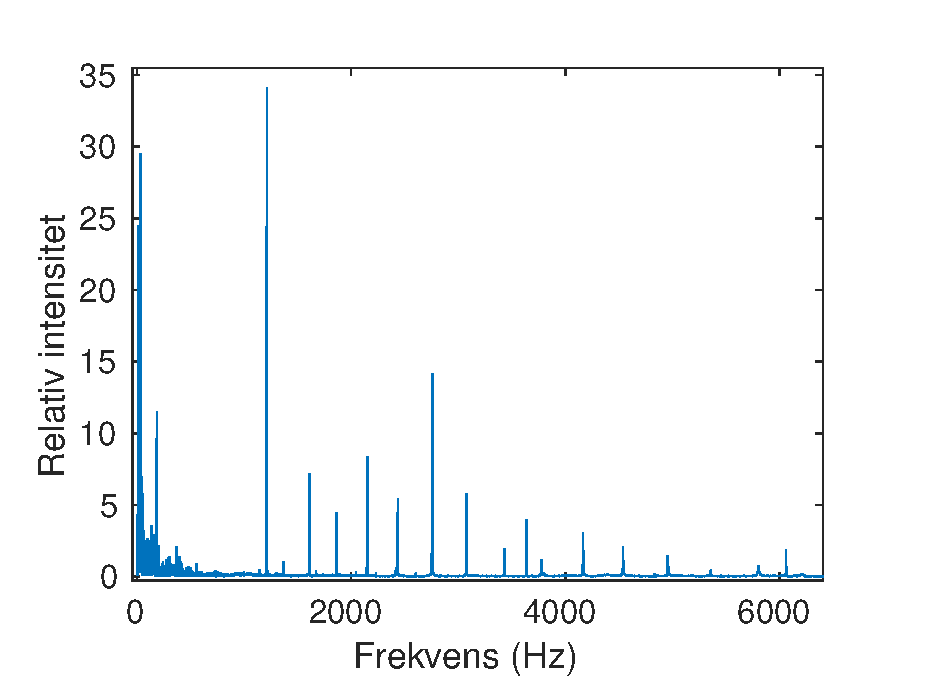
\includegraphics[width = 0.5\textwidth]{matlab/frekvensspekter.eps}
	\caption{Frekvensspekter fra 10 sekunders måling av lyden fra den vibrerende messingstaven.}
	\label{fig:frekvensspekter}
\end{figure}

Ved å gjøre en wavelet analyse finner vi figur \ref{fig:wavelet}, som gir en kvalitativ forståelse av dempningen til svingningene ved de forskjellige frekvensene. Dette rettferdiggjør på at vi plukker ut den frekvensen vi gjør, enn bare ved å betrakte frekvensspekteret. 

\begin{figure}[!ht]
	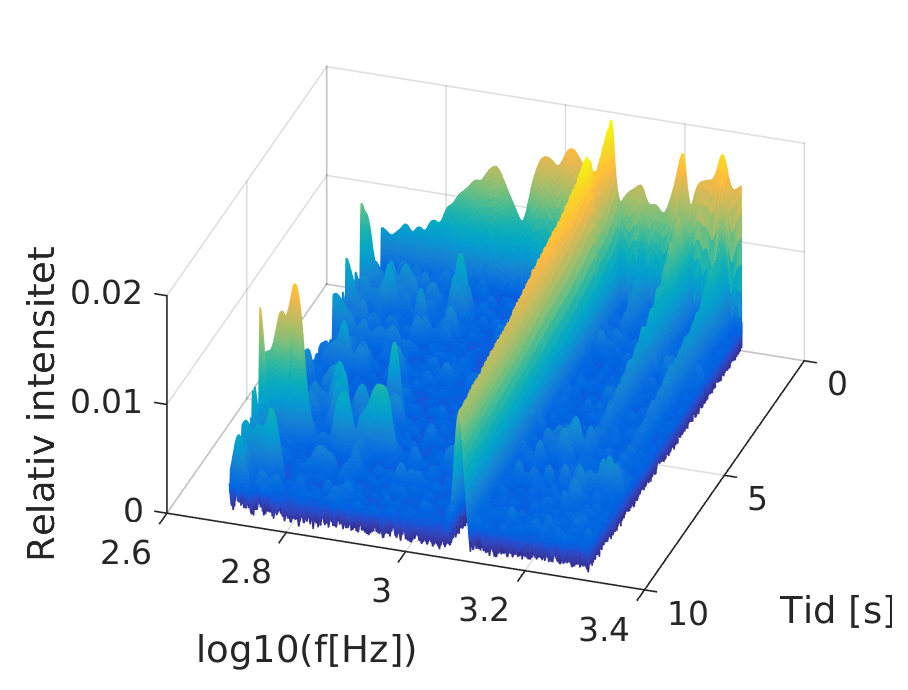
\includegraphics[width = 0.5\textwidth]{matlab/wavelet.eps}
	\caption{Relativ intensitet for lydopptaket plottet som funksjon av tierlogaritmen til frekvens i Hz og tid i sekunder.}
	\label{fig:wavelet}
\end{figure}

Når vi vet dette 

Usikkerheten finner vi til å være $s_E = 0.07$GPa ved å bruke ligning \ref{eq:feilDynamisk}. Dette gir oss en elastisitetsmodul på

\begin{equation}
	E = 103.49\pm0.07\text{GPa}
\end{equation}

\subsection{Sammenligning av resultatene}
Differansen for de to estimatene vi har funnet er 

\begin{equation}
	D = 104.57-103.49\text{GPa} = 1.08\text{GPa} 
\end{equation}

Usikkerheten for denne differansen er 

\begin{align}
s_D &= D\sqrt{s_{E, \text{defleksjon}}^2+s_{E, \text{dynamisk}}^2}\\
&= 0.34\text{GPa}
\end{align}

Vi får altså at differansen $|D|>2s_D$.
\section{Diskusjon}

\subsection{Kalibrering av lodd}
Vi fikk at loddene ikke avviker i veldig stor grad fra den kalibrerte verdien vi fant. Det kunne vært lurt å gjøre flere målinger for kalibreringen for å få en mer allsidig kalibreringskurve, men for bruken i denne oppgaven er det ikke veldig nødvendig.

\subsection{Parametre for messingstaven}
Vi kunne fått mer nøyaktige målinger med et målebånd uten slark i festeleddet.

Massen til messingstaven lå et godt stykke over det høyeste kalibreringspunktet vårt. Vi måtte derfor ekstrapolere i forhold til de verdiene vi hadde å kalibrere med. Dette fører til større usikkerheter enn om vi hadde interpolert, kanskje også større usikkerhet enn det som er benyttet.

Målingene for diameteren er nok det som vil være vanskeligst å forbedre ettersom de allerede er gjort med et mikrometer, som er et ganske nøyaktig instrument for å måle lengde. Samtidig er diameteren en av de faktorene som gir en ganske stor usikkerhet.

\subsection{Defleksjon av messingstav}
Måleuret viser ganske nøyaktige verdier, og er nok ikke en veldig stor kilde til usikkerhet i seg selv. Målingene kan bli litt mindre pålitelige hvis det underlaget tuppen av måleuret står ikke befinner seg i det horisontale plan. Dette hadde vi ikke helt kontroll på gjennom forsøket, men vi sjekket at det var korrekt før vi begynte å legge på masse. Det burde være tilstrekkelig.

Et større problem som vi kom på noen dager etter å ha utført eksperimentet, var at vi ikke er sikre på at målingene vi gjorde for defleksjonen ble tatt på midten av stangen. Når vi kom på laben var alt utstyret allerede satt opp, og vi glemte rett og slett å undersøke denne faktoren nærmere. Problemet er at det er vanskeligere å finne en usikkerhet tilknyttet dette ettersom ligningen \eqref{eq:h}, som vi benyttet som grunnlag for å estimere elastisitetsmodulen, gjelder spesielt under denne antagelsen. 

Det bør nevnes at det nok ikke er snakk om mer enn rundt \'en halv centimer forskyvning, ettersom dette er begrenset av at festet må gjennom et relativt lite hull. Dette hjelper likevel ikke så mye på å kvantifisere usikkerheten uten å gå mer i detalj når det gjelder utledningen av ligningen.

\subsection{Dynamisk måling av elastisitetsmodulen}
Det er mulig at måten vi hang opp stangen på kan ha påvirket svingefrekvensen litt. Vi tror likevel dette er en faktor som ikke spiller en veldig stor rolle ettersom opphenget påfører en kraft til messingstaven som er vinkelrett på bølgenes bevegelsesretning. Usikkerheten i estimatet av elastisitetsmodulen forbedres også mer ved å redusere usikkerheten for målingen av diameteren enn for frekvensen, så det er mindre interessant å undersøke hvordan målingen av stavens svingefrekvens kan forbedres. Dette er selvfølgelig under antagelsen om at usikkerheten til frekvensen stemmer, men vi kunne nok ha benyttet en litt større usikkerhet grunnet at målingen var sterkt tidsvarierende i starten.

\subsection{Sammenligning av resultater}
Ettersom absoluttverdien til differansen mellom estimatene av elastisitetsmodulen for de forskjellige verdiene var større enn det dobbelte av usikkerheten så kan vi med stor sannsynlighet si at differansen ikke skyldes usikkerhet i målingene. Det er altså stor sannsynlighet for at vi har å gjøre med en systematisk feil, grunnet feil oppsett av utstyret.

Det største problemet er mest sannsynlig at vi ikke hadde helt kontroll på plasseringen av måleuret i forhold til at det skulle vært plassert midt mellom hvilepunktene på stangen for målingene av defleksjon for messingstaven. 

\section{Konklusjon}
Vi fant to verdier for samme elastisitetsmodul som hadde en forskjell på omtrent 1\%. Dette var mer enn dobbelt så mye som usikkerheten vi fant. Dette tyder på at de med stor sannsynlighet er gjort feil under målingene som ikke har med måleusikkerhet å gjøre. 

For disse eksperimentene virker det som om plasseringen av måleuret, for måling av defleksjon, var det som førte til størst usikkerhet i forhold til oppsettet. Det kan dermed virke som om det er her den antatte systematiske feilen, som spiller den største rollen, ligger.

Dette tatt i betraktning er det stor sannsynlighet for at elastisitetsmodulen estimert ved den dynamiske metoden er nærmest den riktige verdien. Dette forsterkes av at den estimerte usikkerheten for den dynamiske metoden også er en femtedel av den vi fant for defleksjonsmetoden. Vi kan dermed konkludere med at vårt beste estimat for elastisitetsmodulen er $E = 103.5\pm0.1\text{GPa}$.

\printbibliography
\clearpage
\onecolumn
\appendix


%\section{Matlab-script}

\end{document}
